\documentclass[10 pt,
handout
]{beamer}
\setbeamertemplate{subsection in toc}[subsections numbered]
\usetheme{metropolis}
\usepackage{amsthm}
\usepackage[T1]{fontenc}
\usepackage{lmodern} %For \pounds
\usepackage[sortcites = true, backend=bibtex, style=numeric, url = false]{biblatex} % for bibliography
\usepackage{physics}
\addbibresource{refs.bib}

\theoremstyle{plain} % insert bellow all blocks you want in italic
% to number according to section
\newtheorem{proposition}{Proposition}[section]
\theoremstyle{definition} % insert bellow all blocks you want in normal text
\newtheorem{Def}{Definition}[section] % to number according to section
\newtheorem*{idea}{Proof idea} % no numbered block

\title{Geometría Multisimpléctica, el marco para Teorías Clásicas de Campos}
\subtitle{Seminario de doctorandos}
\author{Rubén Izquierdo-López}
\institute{ICMAT-UCM}
\date{19 September, 2024}

\begin{document}
    \setbeamercolor{background canvas}{bg=white}
    \begin{frame}[plain]
        \titlepage
    \end{frame}
    
    \begin{frame}
        \frametitle{Structure of the talk}
       \tableofcontents
    \end{frame}

    %Section: Preliminaries
    \section{Jet bundles}

\begin{frame}
    \frametitle{The geometry of the first jet bundle}
    
\end{frame}
    
    %Section: The geometry of Calculus of variations
    \section{\bf The geometry of calculus of variations}
\subsection{The geometric setting}
\begin{frame}
    \frametitle{The geometric setting I}
    \begin{center}
        {\large \bf What to minimize/maximize? \alert{Sections!}}
    \end{center}
    Fixed some fibered manifold $$Y \xrightarrow{\pi_{YX}} X \,\, \text{with coordinates } (x^\mu, y^i) \mapsto x^\mu,$$
    we want to find a section $$\phi: X \rightarrow Y,\,\,  (x^\mu) \mapsto (x^\mu, y^i = \phi^i(x^\mu))$$
    minimizing/maximizing the functional $$\mathcal{J}[\phi] = \int_X L\left (x^\mu, \phi^i(x^\mu), \pdv{\phi^i}{x^\mu}, \pdv{\phi^i}{x^\mu}{x^\nu},\dots\right ) d^n x.$$
    We will focus on \alert{first order} theories,
    $$\mathcal{J}[\phi] = \int_X L\left (x^\mu, \phi^i(x^\mu), \pdv{\phi^i}{x^\mu} \right ) d^n x.$$ 
\end{frame}

\begin{frame}
    \frametitle{The geometric setting II}
    We can interpret  $$L\left (x^\mu, \phi^i(x^\mu), \pdv{\phi^i}{x^\mu} \right ) d^n x$$
    as an $n$-form on the first jet bundle $$J^1 \pi_{YX} \text{ with coordinates } (x^\mu, y^i, z^i_\mu).$$ We 
    call it \alert{the Lagrangian density} $$\mathcal{L} = L(z^\mu, y^i, z^i_\mu) d^nx.$$ We can rewrite the action as 
    $$\mathcal{J}[\phi] = \int_X (j^1 \phi)^\ast \mathcal{L}.$$
\end{frame}

\begin{frame}
    \centering
    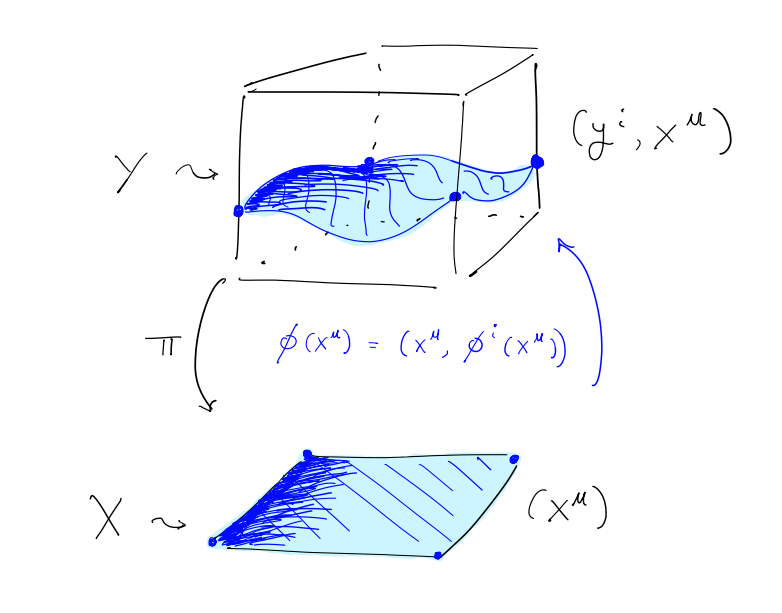
\includegraphics[width = 250pt]{Images/Variational_problem.PNG}
    $$\mathcal{J}[\phi] = \int_X (j^1\phi)^\ast \mathcal{L},$$
    where $\mathcal{L} \in \Omega^n(J^1  \pi_{YX})$ is the Lagrangian dentisy.
\end{frame}

\subsection{The Euler-Lagrange equations}
\begin{frame}
    \frametitle{The Euler-Lagrange equations I}
    If $\phi$ is a minimizer/maximizer (more generally, \alert{stationary section}), 
    $$\dv{t}\bigg |_{t = 0} \mathcal{J}[\textcolor{red}{\phi_t}] = 0, \, \forall \text{ variation } \textcolor{red}{\phi_t}.$$
    \begin{center}
        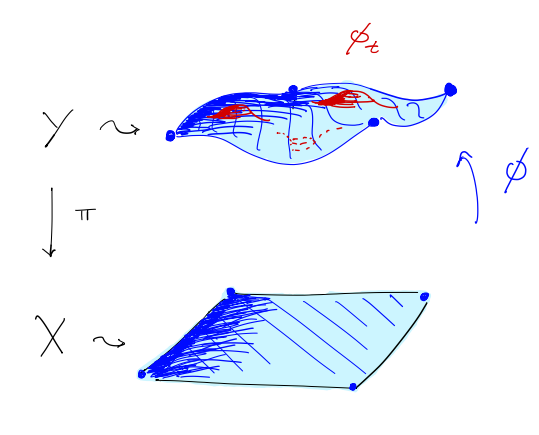
\includegraphics[width = 210pt]{Images/Variations.PNG}
    \end{center}
\end{frame}

\begin{frame}
    \frametitle{The Euler-Lagrange equations II}
    Equivalently, $$0 = \int_X \dv{t}\bigg |_{t = 0} (j^1\textcolor{red}{ \phi_t})^\ast \mathcal{L}.$$
    Locally, we get $$\pdv{L}{y^i} = \dv{x^\mu} \left ( \pdv{L}{z^i_\mu} \right ).$$ 
    \begin{center}
        {\large \bf What about \alert{intrinsic} Euler-Lagrange equations?}
    \end{center}
    If we define
    $$\textcolor{red}{\xi} := \dv{t}\bigg |_{t = 0} \textcolor{red}{\phi_t} = \xi^i \pdv{y^i} \in \mathfrak{X}(Y),$$
    $$\textcolor{red}{\xi^{(1)}} := \dv{t}\bigg |_{t = 0} j^1\textcolor{red}{\phi_t} = \xi^i \pdv{y^i} + \left(\pdv{\xi^i}{x^\mu} + \pdv{x^i}{y^j} z^j_\mu \right) \pdv{z^j_\mu}\in \mathfrak{X}(J^1 \pi_{YX}).$$
\end{frame}

\begin{frame}
    \frametitle{The Euler-Lagrange equations III}
    If we define
    $$\textcolor{red}{\xi} := \dv{t}\bigg |_{t = 0} \textcolor{red}{\phi_t} = \xi^i \pdv{y^i} \in \mathfrak{X}(Y),$$
    $$\textcolor{red}{\xi^{(1)}} := \dv{t}\bigg |_{t = 0} j^1\textcolor{red}{\phi_t} = \xi^i \pdv{y^i} + \left(\pdv{\xi^i}{x^\mu} + \pdv{x^i}{y^j}
     z^j_\mu \right) \pdv{z^j_\mu}\in \mathfrak{X}(J^1 \pi_{YX}),$$
    
    $$0 = \dv{t}\bigg |_{t = 0} \mathcal{J}[\textcolor{red}{\phi_t}] = \int_X (j^1 \phi)^\ast \pounds_{ \textcolor{red}{\xi^{(1)}}}
     \mathcal{L}, \, \text{for every vertical } \textcolor{red}{\xi} \in \mathfrak{X}(Y)$$
    Applying Stokes' Theorem
    $$0 = \int_X (j^1 \phi)^\ast  \iota_{ \textcolor{red}{\xi^{(1)}}}
     d \mathcal{L} + \int_X d \iota_{ \textcolor{red}{\xi^{(1)}}}
     \mathcal{L} = \int_X (j^1 \phi)^\ast  \iota_{ \textcolor{red}{\xi^{(1)}}}
     d \mathcal{L}.$$
\end{frame}

\begin{frame}
    \frametitle{The Euler-Lagrange equations IV}
    $$0 = \int_X (j^1 \phi)^\ast  \iota_{ \textcolor{red}{\xi^{(1)}}}
     d \mathcal{L}\,\, \text{for every vertical } \textcolor{red}{\xi} \in \mathfrak{X}(Y).$$
    \alert{Does not yield equations.}
    \begin{center}
        {\large \bf \alert{Idea}: modify $\mathcal{L}$}
    \end{center}
    We want to find an $n$-form $\Theta_\mathcal{L}$ satisfying $$(j^1 \phi)^\ast \mathcal{L} = (j^1 \phi)^\ast \Theta_\mathcal{L}$$
    such that $\phi$ is an stationary field of the action if and only if
    $$0 = \int_X (j^1 \phi)^\ast  \iota_{ \textcolor{blue}{\eta}}
     d \Theta_\mathcal{L}\,\, \text{for every } \textcolor{blue}{\eta} \in \mathfrak{X}(J^1 \pi_{YX}).$$
\end{frame}

\begin{frame}
    \frametitle{The Euler-Lagrange equations V}
    \begin{proposition} There is such $\Theta_\mathcal{L}$, and can be intrinsically defined (using the geometry of $J^1 \pi_{YX}$).
    \end{proposition}
    Locally, 
    $$\Theta_\mathcal{L} =  \pdv{L}{z^i_\mu}  dy^i \wedge d^{n-1}x_\mu - \left( \pdv{L}{z^i_\mu}z^i_\mu - L \right) d^n x$$
    and it is called \alert{the Poincaré-Cartan form}.

    \begin{corollary}[Intrinsic Euler-Lagrange equations]
        A field $\phi:X \rightarrow Y$ is stationary if and only if it satifies
        $$(j^1 \phi)^\ast \iota_{\textcolor{blue}{\eta}} d\Theta_\mathcal{L} = 0, \,\,\text{for every } \textcolor{blue}{\eta} \in \mathfrak{X}(J^1 \pi_{YX}).$$
    \end{corollary}
\end{frame}

\begin{frame}
    \frametitle{Looking for solutions}
    To find solutions, we can look for distributions on $J^1 \pi_{YX} \rightarrow$ such that an integral
    section of such this distribution $\sigma: X \rightarrow J^1 \pi_{YX}$ satisfies $$\sigma^\ast \iota_\eta \Omega_\mathcal{L} = 0, \forall \eta \in \mathfrak{X} (J^1 \pi_{YX}).$$
    We can define such distributions via decomposable $n$-multivector fields $$U = X_1 \wedge \cdots \wedge X_n.$$
    \begin{center}
        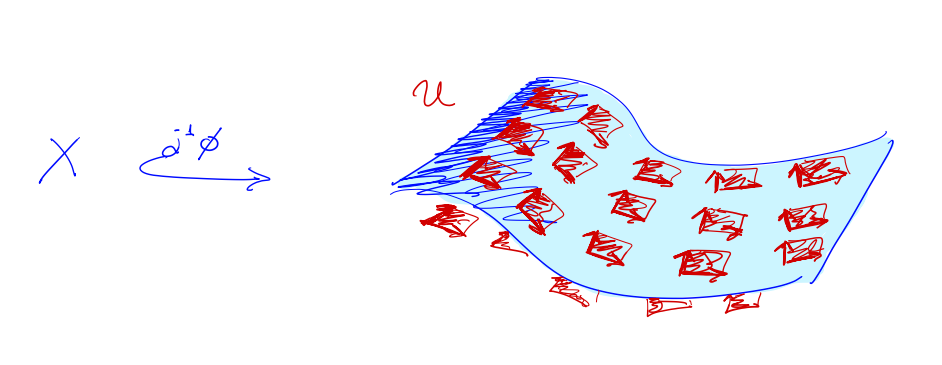
\includegraphics[height = 100pt]{Images/Multivector_multisymplectic.PNG}
    \end{center} 
    Then, being stationary is characterized by $\iota_U \Omega_\mathcal{L} = 0$.
\end{frame}

\begin{frame}
    \frametitle{Disclaimer}
    Giving such a multivector field $U$ does not immediately give a solution:
    \begin{itemize}
        \item We need to make sure that the corresponding distribution is integrable.
        \item Even if it is integrable, it may not be holonomic. That is, that the corresponding 
        integral section $\sigma: X \rightarrow J^1 \pi_{YX}$ could fail to be the jet lift of some section $$\phi: X \rightarrow Y.$$
        When $\mathcal{L}$ is \alert{regular,} this is not an issue.
        \item Even if it satisfies the previous conditions, there may not exist global sections of $Y \xrightarrow{\pi_{YX}} X$.
    \end{itemize}
\end{frame}

\begin{frame}
    \frametitle{Summary}
    \begin{itemize}
        \item Fields, denoted by $\phi$, are sections of a fibered manifold $Y \xrightarrow{\pi_{YX}} X.$
        \item A first order variational problem is defined through a Lagrangian density $\mathcal{L}$ 
         on $J^1 \pi_{YX}$ (which defines an $n$-form on $X$ at each point), and the action can be expressed as
        $$\mathcal{J}[\phi] = \int_X (j^1 \phi)^\ast \mathcal{L}.$$
        \item If we define the \alert{multisymplectic form} as $$\Omega_\mathcal{L} := -d \Theta_\mathcal{L},$$
        stationary fields are characterized by $$(j^1 \phi)^\ast \iota_{\eta} \Omega_\mathcal{L} = 0, \,\, \text{for every } \eta \in \mathfrak{X}(J^1 \pi_{YX}).$$
        In particular, we can look for decomposable horizontal $n$-multivector fields $U$ satisfying $$\iota_U \Omega_\mathcal{L} = 0.$$
    \end{itemize}
\end{frame}


    %Section: Multisymplectic Geometry
    \section{\bf Multisymplectic geometry}

\subsection{Basic definitions}
\begin{frame}
    \frametitle{Basic definitions I}
    \begin{definition} A \alert{multisymplectic manifold} of order $n$ is a pair $(M, \omega)$, where $M$
        is a smooth manifold, and $\omega$ is a closed $(n+1)-$form.
    \end{definition}
    An immediate example is the bundle of $n$-forms on a manifold $Q$. $$M:= \bigwedge^n T^\ast Q \xrightarrow{\tau} Q$$ has 
    a canonical $n$-form, 
    $$\Theta|_{\alpha}(v_1, \dots, v_n) := \alpha(\tau_\ast v_1, \dots, \tau_\ast v_n)$$ and
    $$\Omega := - d  \Theta$$ defines a multisymplectic structure on $M$. 
\end{frame}

\begin{frame}
    \frametitle{Basic definitions II}
    \begin{Def} Let $(M, \omega)$ be a multisymplectic manifold of order $n$. A $q$-multivector field $U$ on $M$ ($q \leq n$) is
        called \alert{Hamiltonian} if $$\iota_U \omega = d \alpha,$$ for certain $(n - q)$-form $\alpha$, which will also
        be called \alert{Hamiltonian}.
    \end{Def}
    \begin{itemize}
        \item Top degree Hamiltonian multivector fields ($n$-multivector fields) represent \alert{solutions} to the variational problem, 
        $$\iota_U \omega  = dH, H \in C^ \infty(M).$$
        \item Hamiltonian vector fields $X \in \mathfrak{X}(M)$ are \alert{symmetries,} $\pounds_X \omega = 0$ and the corresponding
        $(n-1)-$form can be thought of as the \alert{Noether current} of the symmetry.
    \end{itemize}
\end{frame}

\subsection{Noether's Theorem}
\begin{frame}
    \frametitle{Noether's Theorem I}
    Given a Hamiltonian function $H$, and a top degree decomposable multivector field $U$ such that 
    $$\iota_U \omega = dH,$$ let $$j: \Sigma \hookrightarrow M$$ be an $n$-dimensional integral submanifold of $U$ (which can be thought of as a distribution).
    \begin{center}
        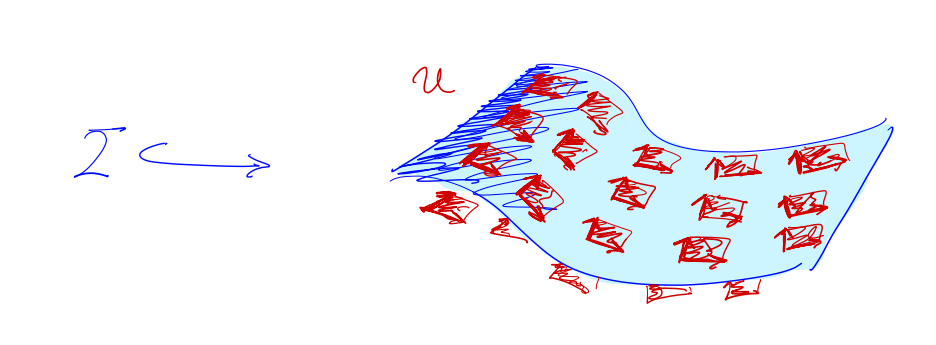
\includegraphics[height = 100pt]{Images/Multivector_variations.PNG}
    \end{center} 
\end{frame}

\begin{frame}
    \frametitle{Noether's Theorem II}
    \begin{theorem}Let $X$ be a Hamiltonian vector field and $\alpha$ the corresponding $(n-1)$-form (the current), $$\iota_X \omega = d \alpha.$$
        Then, if $X$ is a symmetry of $H$, that is, $$X(H) = 0,$$ $\alpha$ is a \alert{conserved current} on $\Sigma,$ this means
        $d(j^\ast \alpha) = 0.$
    \end{theorem}
    \begin{proof} Indeed,
        $$(d\alpha)(U) = \iota U \iota_X \Omega = (-1)^n \iota_X \iota_U \Omega = (-1)^n X(H) = 0.$$
    \end{proof}
\end{frame}

\begin{frame}
    \frametitle{Noether's Theorem III}
    \begin{center}
        {\large \bf What does \alert{conserved} means here?}
    \end{center}
    \begin{center}
        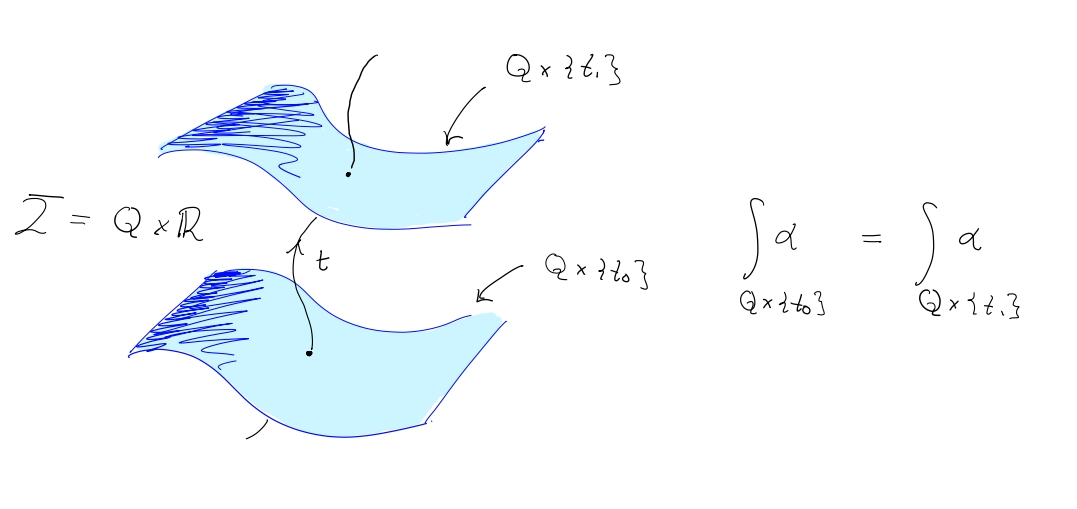
\includegraphics[width = 330 pt]{Images/Noether_current.PNG}
    \end{center}
\end{frame}

\begin{frame}
    \frametitle{Noether's Theorem IV}
    {\large \bf How can we obtain the corresponding current from the symmetry defined by $X$?}
    \begin{theorem} Let $(M, \omega)$ be an \alert{exact} multisymplectic manifold, that is, there exists a \alert{multisymplectic potential}
        $$\omega = - d \theta.$$ Then, if $X$ is a symmetry of $\theta$, $\pounds_X \theta = 0$ (and hence of $\omega$), $$\alpha := - \iota_X \theta$$
        is a current for $X$.
    \end{theorem}
    \begin{proof} Indeed, $$d \alpha = - d \iota_X \theta = - \iota_X d \theta = \iota_X \omega.$$
    \end{proof}
\end{frame}

\subsection{Brackets}
\begin{frame}
    \frametitle{Brackets I}
    \begin{proposition} Let $(M, \omega)$ be a multisymplectic manifold and $\alpha,$ $\beta$ be Hamiltonian forms,
        with Hamiltonian multivector fields, $X$, $Y$, respectively. Then $$\{\alpha, \beta\} := \iota_Y \iota_X \omega$$ is a Hamiltonian form. Its
        Hamiltonian multivector field is $-[X, Y]$ (the Schouten-Nijenhuis bracket).
    \end{proposition}

    \begin{definition}
        Define the \alert{Poisson bracket} of two Hamiltonian forms by $$\{\alpha, \beta\} := -(-1)^{(k - 1 -\operatorname{ord} \alpha )}\iota_Y \iota_X \omega,$$ which is again
        Hamiltonian by the previous proposition.
    \end{definition}
\end{frame}

\begin{frame}
    \frametitle{Brackets II}
    \begin{center}
        {\large \bf What are the properties that $\{\cdot, \cdot\}$ satisfies?}
    \end{center}
    If we define a new degree: $$\deg \alpha:= k -1 - \text{ord} \alpha,$$

    \begin{itemize}
        \item It is \alert{\textit{graded-skew-symmetric}}, that is, $$\{\alpha, \beta\} = (-1)^{\deg \alpha\deg \beta} \{\beta, \alpha\}.$$
        \item Its satisfies \alert{\textit{graded-Jacobi identity}} (up to an exact form) 
        $$(-1)^{\deg \alpha \deg \gamma}\{\{\alpha, \beta\}, \gamma\} + \text{cycl.} = \text{exact term}$$
    \end{itemize}
\end{frame}

\begin{frame}
    \frametitle{Brackets III}
    \begin{theorem} Let $(M, \omega)$ be a multisymplectic manifold. Then, the space of all Hamiltonian forms 
        \alert{modulo exact forms} is a graded Lie algebra.
    \end{theorem}
    Some remarks:
    \begin{itemize}
        \item When restricted to the subspace of forms of $\deg \alpha = 0$, that is, $\operatorname{alpha} = k-1$, 
        we have a Lie algebra, \alert{the Lie algebra of currents}.
        \item Some brackets are zero just by degree considerations, more particularly, when $$\deg \alpha + \deg \beta > k -1,$$
        that is, the bracket is trivial when $$\operatorname{ord} \alpha + \operatorname{ord} \beta < k-1.$$
        \item Dynamics can be characterized by this {Poisson bracket}. Indeed, fixed a Hamiltonian, an $n$-
        multivector field $U$ is a solution ($\iota_U \omega = dH$) if $$\{\alpha, H\} = (d \alpha)(U).$$
    \end{itemize}
\end{frame}

\subsection{...and more!}
\begin{frame}
    \frametitle{...and more!}
    Multisymplectic geometry is a very active area of research, and there has been a lot of interest
    in generalizing classical results from symplectic geometry to the multisymplectic setting.
    \begin{itemize}
        \item Reduction by symmetries.
        \item Coisotropic reduction.
        \item Constraint analysis.
        \item Darboux-like Theorems.
        \item Is everything a Lagrangian submanifold? (Weinstein's creed)
        \item Alogue to Poisson geometry and Dirac geometry (work in progress...).
    \end{itemize}
\end{frame}

\begin{frame}
    \frametitle{Summary}
    \begin{itemize}
        \item Multisymplectic geometry gives an abstract formulation of field theories (calculus of variations).
        \item We can talk about the dynamics and conserved quantities with Hamiltonian multivector fields and forms.
        \item We can prove Noether's Theorem in this formalism.
        \item Hamiltonian forms are endowed with a graded Lie algebra structure (when
        quotiented by exact forms) which yields a Lie algebra when restricted to currents,
        $(n-1)-$forms.
    \end{itemize}
\end{frame}

    %Section: Examples
    \section{\bf Examples}

\subsection{Classical Mechanics}
\begin{frame}
    \frametitle{Classical Mechanics I}
    We recover Classical Mechanics by taking the bundle 
    $$\mathbb{R} \times Q \xrightarrow{\pi} \mathbb{R}.$$ 
    Then, a section is just a curve $\gamma: \mathbb{R} \rightarrow Q.$
    \begin{center}
        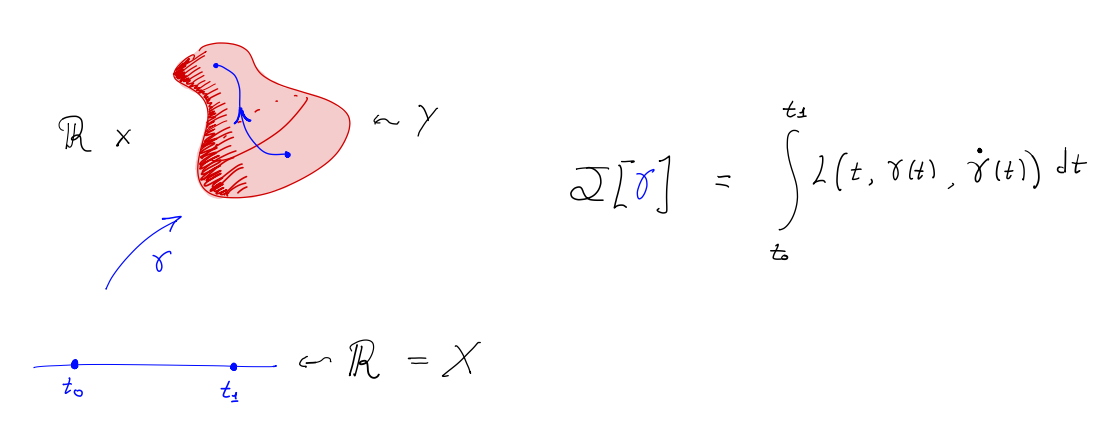
\includegraphics[width = 300pt]{Images/Classical_Mechanics.PNG}
    \end{center}
\end{frame}

\begin{frame}
    \frametitle{Classical Mechanics II}
    The jet bundle:
    $$J^1 \pi = \mathbb{R} \times TQ,$$
    and the \alert{Poincaré-Cartan} form fixed a Lagrangian (which will be identified with a function) $$L : \mathbb{R} \times TQ \rightarrow \mathbb{R}$$ is 
    $$\theta_L = \pdv{L}{\dot{q}^i}d \dot{q}^i - \left(\pdv{L}{\dot{q}^i} \dot{q}^i - L \right) dt.$$
    Dyanmics are vector fields $X$ satisfying 
    \begin{itemize}
        \item \textit{Stationary condition}, $\iota_X d \theta_L = 0.$
        \item \textit{Normalization}, $dt(X) = 1.$
    \end{itemize}
    We recover \alert{cosymplectic} geometry!
\end{frame}

\begin{frame}
    \frametitle{Classical Mechanics III}
    What about Noether Theorem?
    Suppose $L$ $t$-invariant. Then, time translations $\pdv{t}$ define a symmetry of the corresponding multisymplectic form.
    Hence, by previous considerations, $\iota_{\pdv{t}} \theta_L$ is an \alert{conserved current}, that is, a \alert{conserved quantity}.  
    Locally, $$\iota_{\pdv{t}} \theta_L = \pdv{L}{\dot{q}^i} \dot{q}^i - L = H,$$
    obtaining conservation of energy.
\end{frame}

\subsection{Hyperelastic materials}
\begin{frame}
    \frametitle{Hyperelastic materials I}
    We will give an example of hyperelastic dynamics in a fixed background.
    \begin{itemize}
        \item Fix a \alert{body} $(B, G), \rho$, where $B$ is a smooth manifold, $G$ is a Riemannian metric on $B$, and $\rho$ is the mass density.
        \item Fix a background manifold $(M, g)$, with $M$ a smooth manifold and $g$ a Riemannian metric on $B$.
    \end{itemize}
    Dynamics of $B$ on $M$ are time-dependent embeddings $$\phi_t : B \rightarrow M.$$
    We model these embeedings as \alert{fields} $$Y \xrightarrow{\pi} X.$$
\end{frame}

\begin{frame}
    \frametitle{Hyperelastic materials II}
    \begin{itemize}
        \item $X := \mathbb{R} \times B.$
        \item $Y := \mathbb{R} \times B \times M.$
        \item The \alert{projection} $\pi$ is the trivial choice.
    \end{itemize}
    
    There is an \alert{issue}:
    \begin{itemize}
        \item Arbitrary fields of the previous bundle $\phi: X \rightarrow Y$ \textit{do not} necessarily correspond to
        time-dependent embeddings.
    \end{itemize}
    But not for long... 
    \begin{itemize}
        \item Nevertheless, we can still apply the theory developed because embeddings are stable under local perturbations (variations).
    \end{itemize}
\end{frame}

\begin{frame}
    \frametitle{Hyperelastic materials III}
    \begin{center}
        {\large \bf What is the \alert{Lagrangian}?}
    \end{center}
    \alert{Notation}:
    \begin{itemize}
        \item Coordinates on $B$ are denoted by $(x^i) = x^1, \dots, x^{n-1}.$
        \item When adding the time coordinate $t = x^0$, we get coordinates $(x^\mu)$ on $X$.
        \item Coordinates on $M$ are denoted by $(y^a)$.
    \end{itemize}
    Then, the \alert{Lagrangian} is:
    \begin{align*}
        \mathcal{L} &= \mathbb{K} - \mathbb{P}\\
        &= \frac{1}{2} \sqrt{\det G} \rho g_{ab} z^a_0 z^b_0 d^{n+1}x
        - \sqrt{\det G}\rho W(x^\mu, G, g, z^a_i) d^{n+1}x,
    \end{align*}
    where $W$ is the stored energy.
\end{frame}

\begin{frame}
    \frametitle{Hyperelastic materials IV}
    The \alert{Poincaré-Cartan} form is 
    \begin{align*}
        \Theta_\mathcal{L} &= \rho g_{ab}z^b_0 \sqrt{\det G} dy^a \wedge d^n x_0 - \rho \pdv{V}{z^a_i} \sqrt{\det G} dy^a \wedge d^nx_i\\
        & - \left(-\pdv{W}{z^a_i} z^a_i + \frac{1}{2} g_{ab}z^a_0z^b_0 + W\right) \rho \sqrt{\det G} d^{n+1}x
    \end{align*}
    How can we apply Noether's Theorem?
    \begin{itemize}
        \item There is a clear symmetry, \alert{time-invariance}.
        \item Then, the current obtained through the theory is
        \begin{align*}
            \alpha &= -\rho \pdv{W}{z^a_i} \sqrt{\det G} dy^i d^n x_{i0}\\
             &+ \left(\frac{1}{2}g_{ab}z^a_0z^b_0  + W - \pdv{W}{z^a_i} z^a_i\right) \rho \sqrt{\det G} d^{n+1} x_0.
        \end{align*}
    \end{itemize}
\end{frame}

\begin{frame}
    \frametitle{Hyperelastic materials V}
    on holonomic sections it takes the expression
    $$\alpha =\left(  \frac{1}{2} g_{ab}z^a_0z^b_0 + W \right)\rho \sqrt{\det G} d^{n+1} x_0 + \rho \pdv{W}{z^a_i}z^a_0 \sqrt{\det G} d^n x_i$$
    Since $$e = \left(  \frac{1}{2} g_{ab}z^a_0z^b_0 + W \right)\rho \sqrt{\det G}d^{n+1}x_0$$ can be though of as the \alert{energy dentisy}.
    This gives us a conservation law, where $$\rho \pdv{W}{z^a_i}z^a_0 \sqrt{\det G} d^n x_i$$ is the energy flux.
\end{frame}

\begin{frame}
    \frametitle{Final remarks}
    \begin{itemize}
        \item Multisymplectic geometry is a tool that allows us to study variational problems (field theory, Classical Mechanics, 
        some problems in material modelling...)
        \item It is a very active area of research, both from the mathematical and the physical point of view.
        \item Applications to material modelling seem interesnting, have been practically unexplored.
    \end{itemize}
\end{frame}

\begin{frame}
    \nocite{*}
    \printbibliography
\end{frame}

\begin{frame}[plain]
    \begin{center}
        {\Large Thank you for your attention!}
    \end{center}
\end{frame}


\end{document}